\chapter{Optimization of steam generating system}
\label{cha:osgs}
\section{Steam generating subsystem}

In a solar parabolic trough power plant in which intermediate heat-transfer fluid (take oil for instance) is used, heat addition to the working fluid (take water for instance) takes place in three counterflow heat exchangers (steam generator subsystem, SGSS) as shown in \autoref{fig:PTC}. The SGSS consists of preheater, evaporator and superheater. The flow rates of both oil and water remain the same in the three heat exchangers. 
The water has phase change in the three heat exchangers, from liquid to vapor in the evaporator, however, oil remains liquid. The heat capacity of water in each heat exchanger  differs significantly. The heat capacity of oil has no significant difference since no phase change. The heat transfer process is illustrated on \autoref{fig:DeltaTmin}. Large temperature differences exist at the inlets and outlets of the heat exchangers, which leads to large entropy production during the entire heat exchange process.

\begin{figure}[htbp]
\centering
	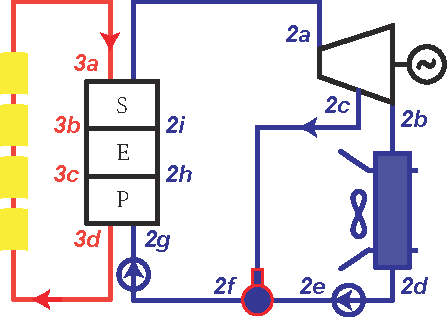
\includegraphics[width = 0.4\columnwidth]{fig/PTC}
	\caption{A typical solar parabolic trough system}
	\label{fig:PTC}
\end{figure}
\begin{figure}[htbp]
\centering
	\includegraphics[width = 0.5\columnwidth]{fig/DeltaTmin}
	\caption{The steam generating process in counterflow heat exchangers}
	\label{fig:DeltaTmin}
\end{figure}

The HTF at $3a$ represents the solar field outlet temperature and at $3d$, the field inlet temperature. The difference between the two can be reduced by increasing the flow rate of HTF through the field.

Since the heat exchangers must always stay a positive temperature difference for heat transfer, the temperature of oil must always be higher than the temperature of water. On the other hand, the temperature of oil should not be much higher than that of the water. Higher oil temperature leads to more heat losses in the solar field hence lower efficiency, more entropy production generated in the heat exchange process. Besides, higher oil temperature brings greater operational risks for the solar system. Setting the appropriate temperature difference between the oil and water is particularly important. The oil temperature must always higher (but not too much higher) than that of the water.

To find out the inlet and outlet temperatures of oil at the solar field, the lowest temperature difference of oil and water is defined as the pinch temperature $\Delta T_{min}$. The temperatures of state points $2h$ and $2i$ are determined by the main pressure of the steam turbine in \autoref{fig:PTC}, and $T_{3b}$ is larger than $T_{3c}$. So state points $3c$ and $2h$, called the pinch points, are set to satisfy the pinch temperature, $T_{3c} - T_{2h} = \Delta T_{min}$. The pinch temperature $\Delta T_{min}$ is usually set to be 10$\sim$20$\,\mathrm{K}$.
It has to be mentioned that the temperature differences $T_{3d} - T_{2g}$ and $T_{3a} - T_{2a}$ worth attention to be larger than $\Delta T_{min}$.

However, even with the chosen pinch temperature $\Delta T_{min}$, the temperature difference during the heat exchange process in SGSS is still large due to the phase change of water. Large temperature differences always exist at the inlet/outlet of the exchangers. As shown in \autoref{fig:DeltaT}, it is a tradeoff to choose a mass flow rate of oil ($\dot{m}_3$). $\dot{m}_3$ affects the slope of curve $3a$-$3b$-$3c$-$3d$. A smaller $\dot{m}_3$ leads to a steeper curve, hence a larger $T_{3a} - T_{2j}$. A larger $\dot{m}_3$ leads to a more gentle curve, hence a larger $T_{3d} - T_{2g}$. The heat transfer processes in SGSS always produce large entropy and exergy losses. In this regard, a new steam generating system to reduce exergy loss is put forward.

\begin{figure}[htbp]
\centering
	\includegraphics[width = 0.5\columnwidth]{fig/DeltaT}
	\caption{The tradeoff to choose $\dot{m}_3$}
	\label{fig:DeltaT}
\end{figure}

\section{Multistage exergy loss reduction system}\label{sec:melrs}
The reason of large temperature differences of the two curves in \autoref{fig:DeltaTmin} is that, the slope of oil curve changes slightly in different heat exchangers (preheater, evaporator and superheater), while the water curve changes dramatically due to large heat capacity $c_p$ differences.

\begin{equation}
  \Delta Q =  c_p\dot{m} \Delta T
\end{equation}

The slope of the curves are determined by $c_p\dot{m}$, $\dot{m}$ can be altered to adjust the slope of the curves despite $c_p$ is unalterable. All the water needs to be heated from supercooled water to superheated steam, which means $\dot{m}_2$ remains the same in the three heat exchangers. The last way is to change $\dot{m}_3$ in the heat exchangers.

\begin{figure}[htbp]
\centering
	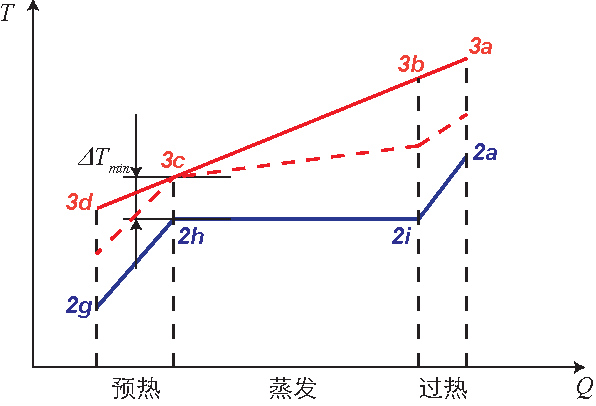
\includegraphics[width = 0.5\columnwidth]{fig/BetterCurve}
	\caption{Change $\dot{m}_3$ in the heat exchangers to reduce the temperature difference}
	\label{fig:BetterCurve}
\end{figure}

As shown in \autoref{fig:BetterCurve}, the oil curve can be changed to the dashed curve. The temperature difference between the water curve and oil curve reduces significantly. Water is heated in three stages and the exergy loss reduces. The corresponding steam generating system is so called Multistage Exergy Loss Reduction System (MELRS).
\autoref{fig:SEP} shows the schematic diagram of the MELRS for comparison with typical solar parabolic trough system in \autoref{fig:PTC}. The solar field in \autoref{fig:PTC} has been divided into three independent sectors. Each sector becomes the heat source of a range for the steam heating process: the first corresponds to overheating, the second to evaporation, and the third to preheating. 
%Each section can be equipped with a thermal storage system to overcome the instability and intermittency of solar energy.
It has to be mentioned that the collectors in the schematic diagram are only used for explanation. The arrangement of these collectors can be in series, in parallel or combination of both.

\begin{figure}[htbp]
\centering
	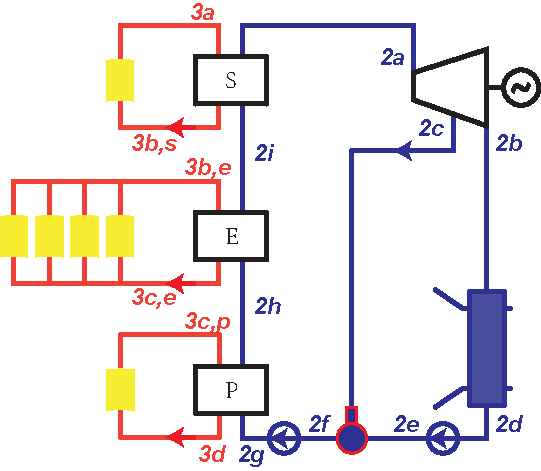
\includegraphics[width = 0.5\columnwidth]{fig/SEP}
	\caption{The schematic diagram of the MELRS}
	\label{fig:SEP}
\end{figure}

To optimize the MELRS, considering the constrain of pinch temperature, temperatures of the oil at the inlet/outlet of the heat exchangers can be set according to following rules:
\begin{eqnarray*}
	&T_{3d} - T_{2g} = \Delta T_{min}\\
   &T_{3c,p} = T_{3c,e} = T_{3c}\\
   &T_{3c} - T_{2h} = \Delta T_{min}\\
	&T_{3b,e} = T_{3b,s} = T_{3b}\\
	&T_{3a} - T_{2a} = \Delta T_{min}
\end{eqnarray*}


A large flow rate of oil in the evaporator $\dot{m}_{3,e}$ can be applied to reduce the temperature $T_{3b}$ hence the temperature differences of the oil and water. However, a large $\dot{m}_{3,e}$ requires more pump power consumption for the oil circuits. Besides, $\dot{m}_{3,e}$ is limited for the limitation of oil velocity in the pipes.

The enthalpy of each state point can be determined by its temperature and pressure.

The optimum oil average temperature in the solar field corresponds to the preheater is
\begin{equation}
  T_{3,p} = (T_{2g} + T_{2h})/2 + \Delta T_{min}
\end{equation}

The optimum oil flow rate in the solar field corresponds to the preheater is
\begin{equation}
  \dot{m}_{3,p} = \dot{m}_{2}(h_{2h} - h_{2g})/(h_{3c} - h_{3d})
\end{equation}

The optimum oil average temperature in the solar field corresponds to the evaporator is
\begin{equation}
  T_{3,e} = (T_{3b} + T_{3c})/2
\end{equation}

The optimum oil flow rate in the solar field corresponds to the evaporator is
\begin{equation}
  \dot{m}_{3,e} = \dot{m}_{2}(h_{2i} - h_{2h})/(h_{3b} - h_{3c})
  \label{eq:m_3e}
\end{equation}

The optimum oil average temperature in the solar field corresponds to the superheater is
\begin{equation}
  T_{3,s} = (T_{3b} + T_{2a} + \Delta T_{min})/2
\end{equation}

The optimum oil flow rate in the solar field corresponds to the superheater is
\begin{equation}
  \dot{m}_{3,s} = \dot{m}_{2}(h_{2a} - h_{2i})/(h_{3a} - h_{3b})
\end{equation}

\section{Comparison}

To find out the effect of MELRS, models of traditional SGSS and proposed MELRS are developed based on the models of the components created in \autoref{cha:Modeling}. 
To clearly find out the influence of oil temperature on the performance of the trough collectors, \autoref{eq:eta_tc} in \autoref{sec:ptc} is used.
%To find out the effect of MELRS, models of traditional SGSS and proposed MELRS are developed based on the models of the components. To clear find out the influence of oil temperature on the performance of the trough collectors, the equation summarized by~\cite{Rovira2011} is used.
%\begin{equation}
%  \eta(T) =  0.69563 + 0.000313T - 0.0000013T^2
%\end{equation}
%where $T$ is the average temperature of the tube. Since the $Nu$ number in the tube is large (about 1$\times$10$^4$), small temperature difference exists between the absorber and oil. So the average oil temperature can be used as the average value of the tube.

The exergy loss caused by a heat exchange process per unit time
\begin{equation}
  \dot{I} = T_{amb} (\sum \dot{m}_os_o - \sum \dot{m}_is_i)
  \label{eq:dot_I}
\end{equation}

\begin{table}[htbp]
	\caption{Main parameters used for SGSS and MELRS}
	\centering
	\begin{tabular}{cccc}
		\toprule
		Parameter		&	Value	&	Parameter		&	Value\\
		\midrule
		$I_r$	&	700$\,\mathrm{W/m^2}$	&	$T_s$		&	613.15$\,\mathrm{K}$\\
		$P_{ge}$	&	6$\times$10$^6\,\mathrm{W}$	&	$p_s$		&	2.35$\times$10$^6\,\mathrm{Pa}$\\
		$\eta_{i,tb}$	&	0.711	&	$p_c$		&	1.5$\times$10$^4\,\mathrm{Pa}$\\
		$\eta_{ge}$	&	0.975	&	$p_{de}$		&	1$\times$10$^6\,\mathrm{Pa}$\\
		$\Delta T_{min}$	&	15$\,\mathrm{K}$	&	&\\		
		\bottomrule
	\end{tabular}
	\label{tab:ptc}
\end{table}

The turbine and deaerator are the same for the two systems (SGSS and MELRS), so that the corresponding state points of water are the same. The main parameters are listed in \autoref{tab:ptc}.

\begin{figure}[htbp]
\centering
	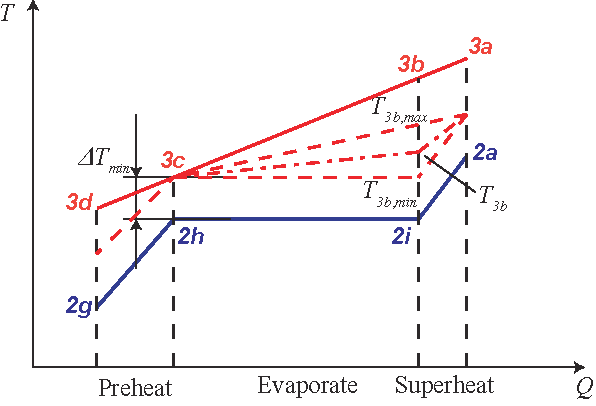
\includegraphics[width = 0.7\columnwidth]{fig/T3b}
	\caption{$T_{3b}$ in the $T$-$Q$ diagram of the heat transfer processes}
	\label{fig:T3b}
\end{figure}

As discussed in \autoref{sec:melrs}, $T_{3b}$ is an undetermined value. \autoref{fig:T3b} shows the minimum and maximum value of it. $T_{3b,min}$ means the limit situation of unlimited flow rate of oil in the evaporator, $T_{3b,min} = T_{3c}$. $T_{3b,max}$ has the traditional effect of temperature differences in the evaporator and superheater, $\dot{m}_{3,e} = \dot{m}_{3,s}$. In our research, $T_{3b}$ is set to be the average value of the two limitations, $T_{3b} = (T_{3b,min} + T_{3b,max}) / 2$.
\begin{equation}
  \dfrac{T_{3b,max}-T_{3c}}{T_{3a} - T_{3c}} = \dfrac{T'_{3b} - T_{3c}}{T'_{3a} - T_{3c}}
\end{equation}

where $T'_{3a}$ and $T'_{3b}$ are the inlet oil temperature of superheater and evaporator in SGSS respectively.
\begin{table}[htbp]
	\caption{Simulation results of SGSS and MELRS}
	\centering
	\begin{tabular}{ccccc}
		\toprule
		& \multirow{2}{*}{SGSS} & \multicolumn{3}{c}{MELRS}\\\cline{3-5}
 &  & $T_{3b,max}$ & $T_{3b}$ & $T_{3b,min}$\\
		\midrule
		$T_{2a}$ & \multicolumn{4}{c}{613.15$\,\mathrm{K}$}\\
		$T_{2i}$ & \multicolumn{4}{c}{493.83$\,\mathrm{K}$}\\
		$T_{2h}$ & \multicolumn{4}{c}{493.83$\,\mathrm{K}$}\\
		$T_{2g}$ & \multicolumn{4}{c}{453.28$\,\mathrm{K}$}\\
		$T_{3c}$ & \multicolumn{4}{c}{508.83$\,\mathrm{K}$}\\
%		$T_{3d}$	&	495.43$\,\mathrm{K}$	&	\multicolumn{3}{c}{468.28$\,\mathrm{K}$}\\
		$T_{3a}$	&	653.15$\,\mathrm{K}$
	&	628.15$\,\mathrm{K}$	&	628.15$\,\mathrm{K}$	&	628.15$\,\mathrm{K}$\\
		$T_{3b}$	&	634.11$\,\mathrm{K}$	&	612.41$\,\mathrm{K}$	&	560.62$\,\mathrm{K}$	&	508.83$\,\mathrm{K}$\\
		$T_{3d}$	&	495.43$\,\mathrm{K}$
	&	468.28$\,\mathrm{K}$	&	468.28$\,\mathrm{K}$	&	468.28$\,\mathrm{K}$\\
%		$T_{3a}$	&	653.15$\,\mathrm{K}$	&	\multicolumn{3}{c}{628.15$\,\mathrm{K}$}\\
		$\dot{m}_{3p}$	&	47.8$\,\mathrm{kg/s}$	&	16.1$\,\mathrm{kg/s}$	&	16.1$\,\mathrm{kg/s}$	&	16.1$\,\mathrm{kg/s}$\\
		$\dot{m}_{3e}$	&	47.8$\,\mathrm{kg/s}$	&	58.6$\,\mathrm{kg/s}$	&	120.8$\,\mathrm{kg/s}$	&	$\infty$\\
		$\dot{m}_{3s}$	&	47.8$\,\mathrm{kg/s}$	&	59.4$\,\mathrm{kg/s}$	&	14.3$\,\mathrm{kg/s}$	&	8.3$\,\mathrm{kg/s}$\\
		$\dot{I}_p$    &    4.80$\times$10$^4\,\mathrm{W}$    	&  2.58$\times$10$^4\,\mathrm{W}$  &	2.58$\times$10$^4\,\mathrm{W}$	&	2.58$\times$10$^4\,\mathrm{W}$\\
		$\dot{I}_e$    &    1.10$\times$10$^6\,\mathrm{W}$    	&  9.68$\times$10$^5\,\mathrm{W}$  &	6.24$\times$10$^5\,\mathrm{W}$	&	2.41$\times$10$^5\,\mathrm{W}$	\\
		$\dot{I}_s$    &    1.81$\times$10$^5\,\mathrm{W}$    	&  1.42$\times$10$^5\,\mathrm{W}$  &	9.19$\times$10$^4\,\mathrm{W}$	&	4.24$\times$10$^4\,\mathrm{W}$\\
		$\dot{I}_{total}$    &    1.33$\times$10$^6\,\mathrm{W}$    &  1.14$\times$10$^6\,\mathrm{W}$  &	7.44$\times$10$^5\,\mathrm{W}$	&	3.10$\times$10$^5\,\mathrm{W}$\\
		$\eta_p$    &    0.699    &	0.703	&    0.703	&	0.703\\
		$\eta_e$    &    0.673    &	0.678	& 0.689	&	0.697\\
		$\eta_s$    &    0.633    &  0.648	&  0.662	&	0.675\\
		$\eta_{overall}$    &    0.670   &	0.676	&    0.686	&	0.695\\
		\bottomrule
	\end{tabular}
	\label{tab:comparison}
\end{table}
%该表格的解释

Simulation results of the four system models are listed in \autoref{tab:comparison}. It can be found that MELRS can effectively reduce the exergy loss of the steam generating process. The exergy loss can be reduced from 14.3\% up to 76.7\% for the three MELRS. The overall thermal efficiency of the solar fields can be improved from 0.9\% up to 3.6\%.

It is worthy pointing that, for the situation $T_{3b} = T_{3b,min}$, when $\dot{m}_{3e} = \infty$, the \autoref{eq:dot_I} is not applicable. The new correlation listed below is applied for the isothermal heat transfer process

\begin{equation}
  \dot{I} = T_{amb} (\frac{Q}{T_{2h}} - \frac{Q}{T_{3c}}) = \frac{QT_{amb}(T_{3c} - T_{2h})}{T_{2h}T_{3c}}
  \label{eq:isothermal}
\end{equation}

where, $Q$ is the heat transferred per unit time in the evaporator.

$T_{2a}$, $T_{2i}$, $T_{2h}$, $T_{2g}$ and $T_{3c}$ are the same for SGSS and different MELRSs for the same water side processes. The different mass flow rates of the oil lead to different oil temperatures in the heat exchangers, and hence different exergy loss. It can be found that the exergy losses in preheaters of MELRSs ($2.58\times 10^4\,\mathrm{W}$) are smaller than that of SGSS ($4.80\times10^4\,\mathrm{W}$). The exergy losses in evaporators of different MELRSs vary greatly, from $9.68\times10^5\,\mathrm{W}$ to $2.41\times10^5\,\mathrm{W}$ for oil flow rate from $58.6\,\mathrm{kg/s}$ to infinity.
Exergy loss in the evaporator takes the largest portion of the steam generating process, which takes about 82.8\%, 85.2\%, 83.8\% and 78.0\% for SGSS and MELRSs separately.
Increasing flow rate of the heating fluid in the steam generating process can effectively reduce the exergy loss.
The exergy losses in superheaters of MELRSs ($1.42\times 10^5\,\mathrm{W}$, $9.19\times 10^4\,\mathrm{W}$ and $4.24\times 10^4\,\mathrm{W}$) are much smaller than that of SGSS ($1.81\times10^5\,\mathrm{W}$) due to large temperature differences in the traditional superheaters.

It can be found that MELRS can effectively reduce exergy loss hence improve the system efficiency compared to traditional SGSS. The thermal efficiency for the corresponding solar field for the preheater ($\eta_p$), evaporator ($\eta_e$) and superheater ($\eta_s$) of MELRSs are higher than that of SGSS (virtual solar fields).
The overall thermal efficiency ($\eta_{overall}$) of the solar field can be improved effectively.

\section{Conclusion}

In this chapter, a novel multistage exergy loss reduction system is proposed to reduce the large exergy loss in traditional solar parabolic trough power plants.
Traditional solar field is divided into three solar fields to provide heat for the preheater, evaporator, and superheater, respectively. Different flow rates in the three solar fields provide the ability to reduce temperature difference for the heat exchange processes.

Smaller temperature difference leads to lower oil temperature and therefore higher solar field thermal efficiency. Besides, the different temperature ranges of different solar fields provide the convenience of the application of different types of collectors.

The analytical model of the steam generating system is developed. A flow control strategy of HTF depending on the analytical system model is derived. Energy and exergy efficiency of the MELRS is analyzed and compared with the SGSS of traditional solar parabolic trough power plant. Result shows that MELRS can effectively reduce the exergy loss in the heating process, and the performance of the plant can be improved. The exergy loss can be reduced from 14.3\% up to 76.7\% for the three typical MELRSs. The overall thermal efficiency of the solar fields can be improved from 0.9\% up to 3.6\%.